\lhead{\emph{Resultados Experimentales}}
\graphicspath{{Imagenes/}} 
\chapter{Resultados Experimentales}

En este capitulo se muestra un ejemplo del an�lisis mediante el uso de tres aplicaciones diferenciando las dos formas que tiene el usuario de brindar datos a la herramienta.\par

\section{Descripci�n de aplicaciones a analizar}

\begin{description}
\item[SendSMS.apk:] Esta aplicaci�n filtra el device ID del usuario a trav�s de un mensaje de texto. Lee el Device ID y a continuaci�n lo a�ade a un intent utilizando el m�todo putExtra(), acto seguido env�a el intent a trav�s del m�todo startActivityForResult() permitiendo a otra aplicaci�n recibirlo y responder. Una vez recibida la respuesta, la aplicaci�n filtra los datos a un mensaje.
\item[Echoer.apk:] Esta aplicaci�n recibe un intent usando el m�todo getIntent(), escribe los datos recibidos en el Log y por ultimo, env�a los datos de vuelta usando setResult().
\item[WriteFile.apk:] Esta aplicaci�n es similar a SendSMS, excepto que lee la ubicaci�n del dispositivo y la fuga a un archivo.
\end{description}
\par

\section{Datos}

\subsection{Jerarqu�a de niveles de seguridad}

En este ejemplo se usaron los niveles de seguridad que muestra la Figura 17. En ella se puede observar a modo de comentario la representaci�n gr�fica del orden generado.\par

\begin{center}
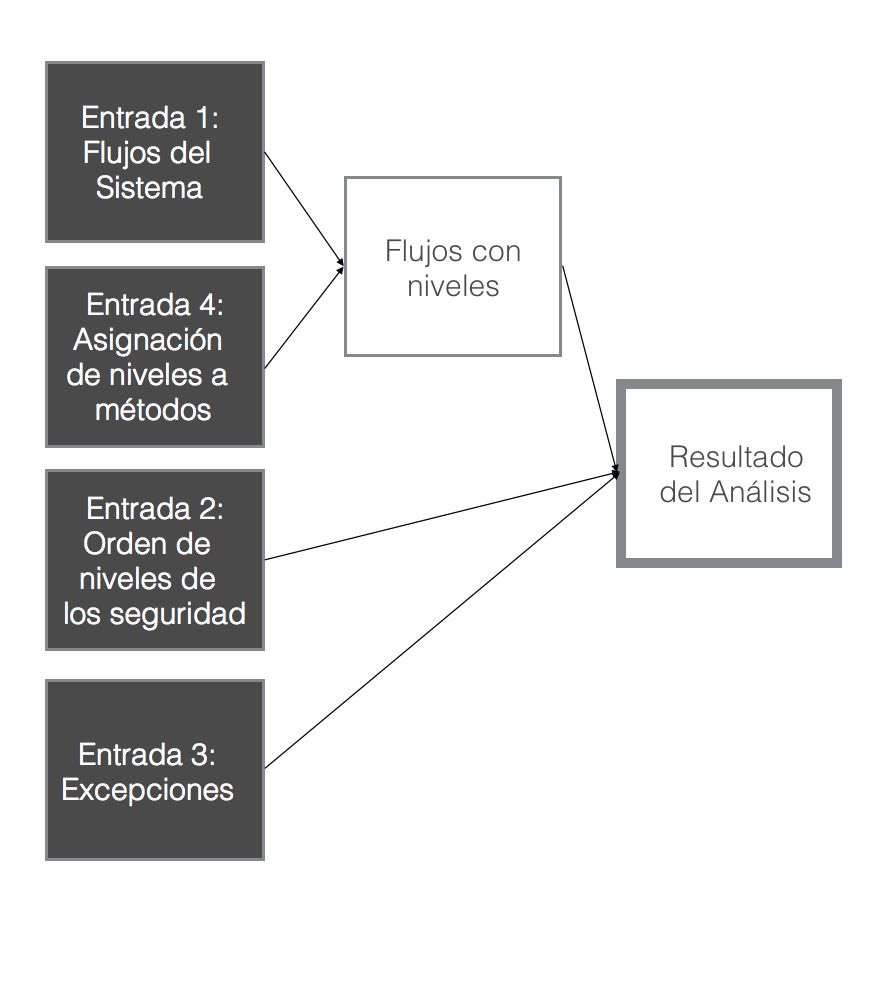
\includegraphics[scale=0.5]{Figura17}
\end{center}

\subsection{Asignaci�n de niveles}

Para mostrar el funcionamiento de la herramienta solo se le asigna niveles a dos categor�as como muestra la Figura 18, ya que, como se ah mencionado con anterioridad, no es necesario darle niveles a todas las categor�as participantes en los flujos de informaci�n, los restantes niveles de seguridad ser�n inferidos por el an�lisis. \par

\begin{center}
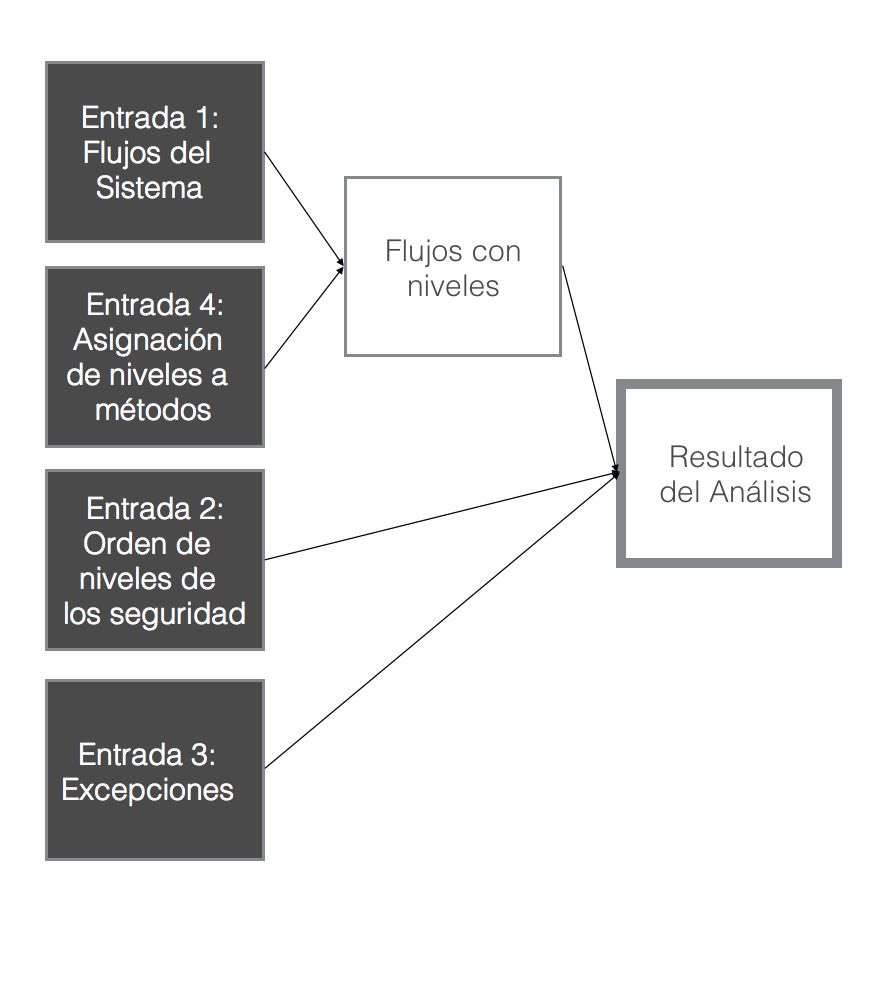
\includegraphics[scale=0.75]{Figura18}
\end{center}

\subsection{Excepciones}

La excepci�n de la Figura 19 hace que se ignore el flujo del device ID del usuario al Log.\par

\begin{center}
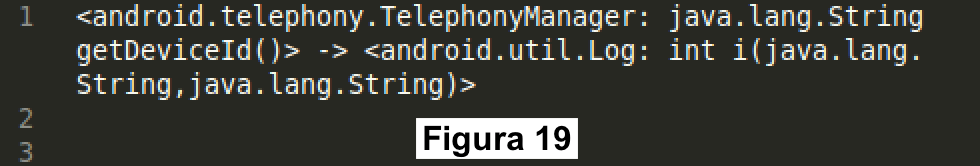
\includegraphics[scale=0.75]{Figura19}
\end{center}

\subsection{Didfail modificado}

La figura 20 muestra los flujos de informaci�n, los m�todos que participan y los niveles de seguridad tiene cada uno asignado.\par

\begin{center}
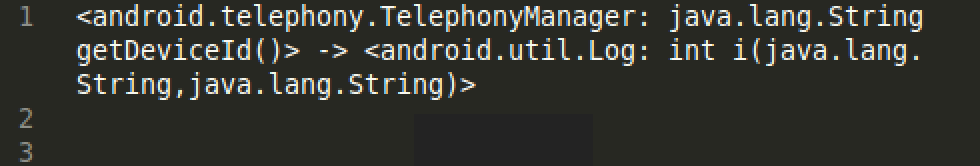
\includegraphics[scale=0.38]{Figura20}
\end{center}

\section{Resultados obtenidos}

Los resultados obtenidos (Figura 21) muestran que no se producen flujos de informaci�n que viole los niveles de seguridad. Adem�s muestra el menor nivel posible, con respecto a los niveles de seguridad, a cada categor�a que no ten�an nivel asignado.\par
La salida tambi�n incluye los Intent lanzados por las aplicaciones. En el conjunto actual de aplicaciones, estos ya fueron utilizados para el an�lisis y no agrega informaci�n en la salida, pero teniendo en cuenta una posible adici�n de otra aplicaci�n al conjunto, el usuario tiene la posibilidad de ver el nivel de la informaci�n que la nueva aplicaci�n puede obtener (en caso de que su archivo manifest as� lo permita).\par

\begin{center}
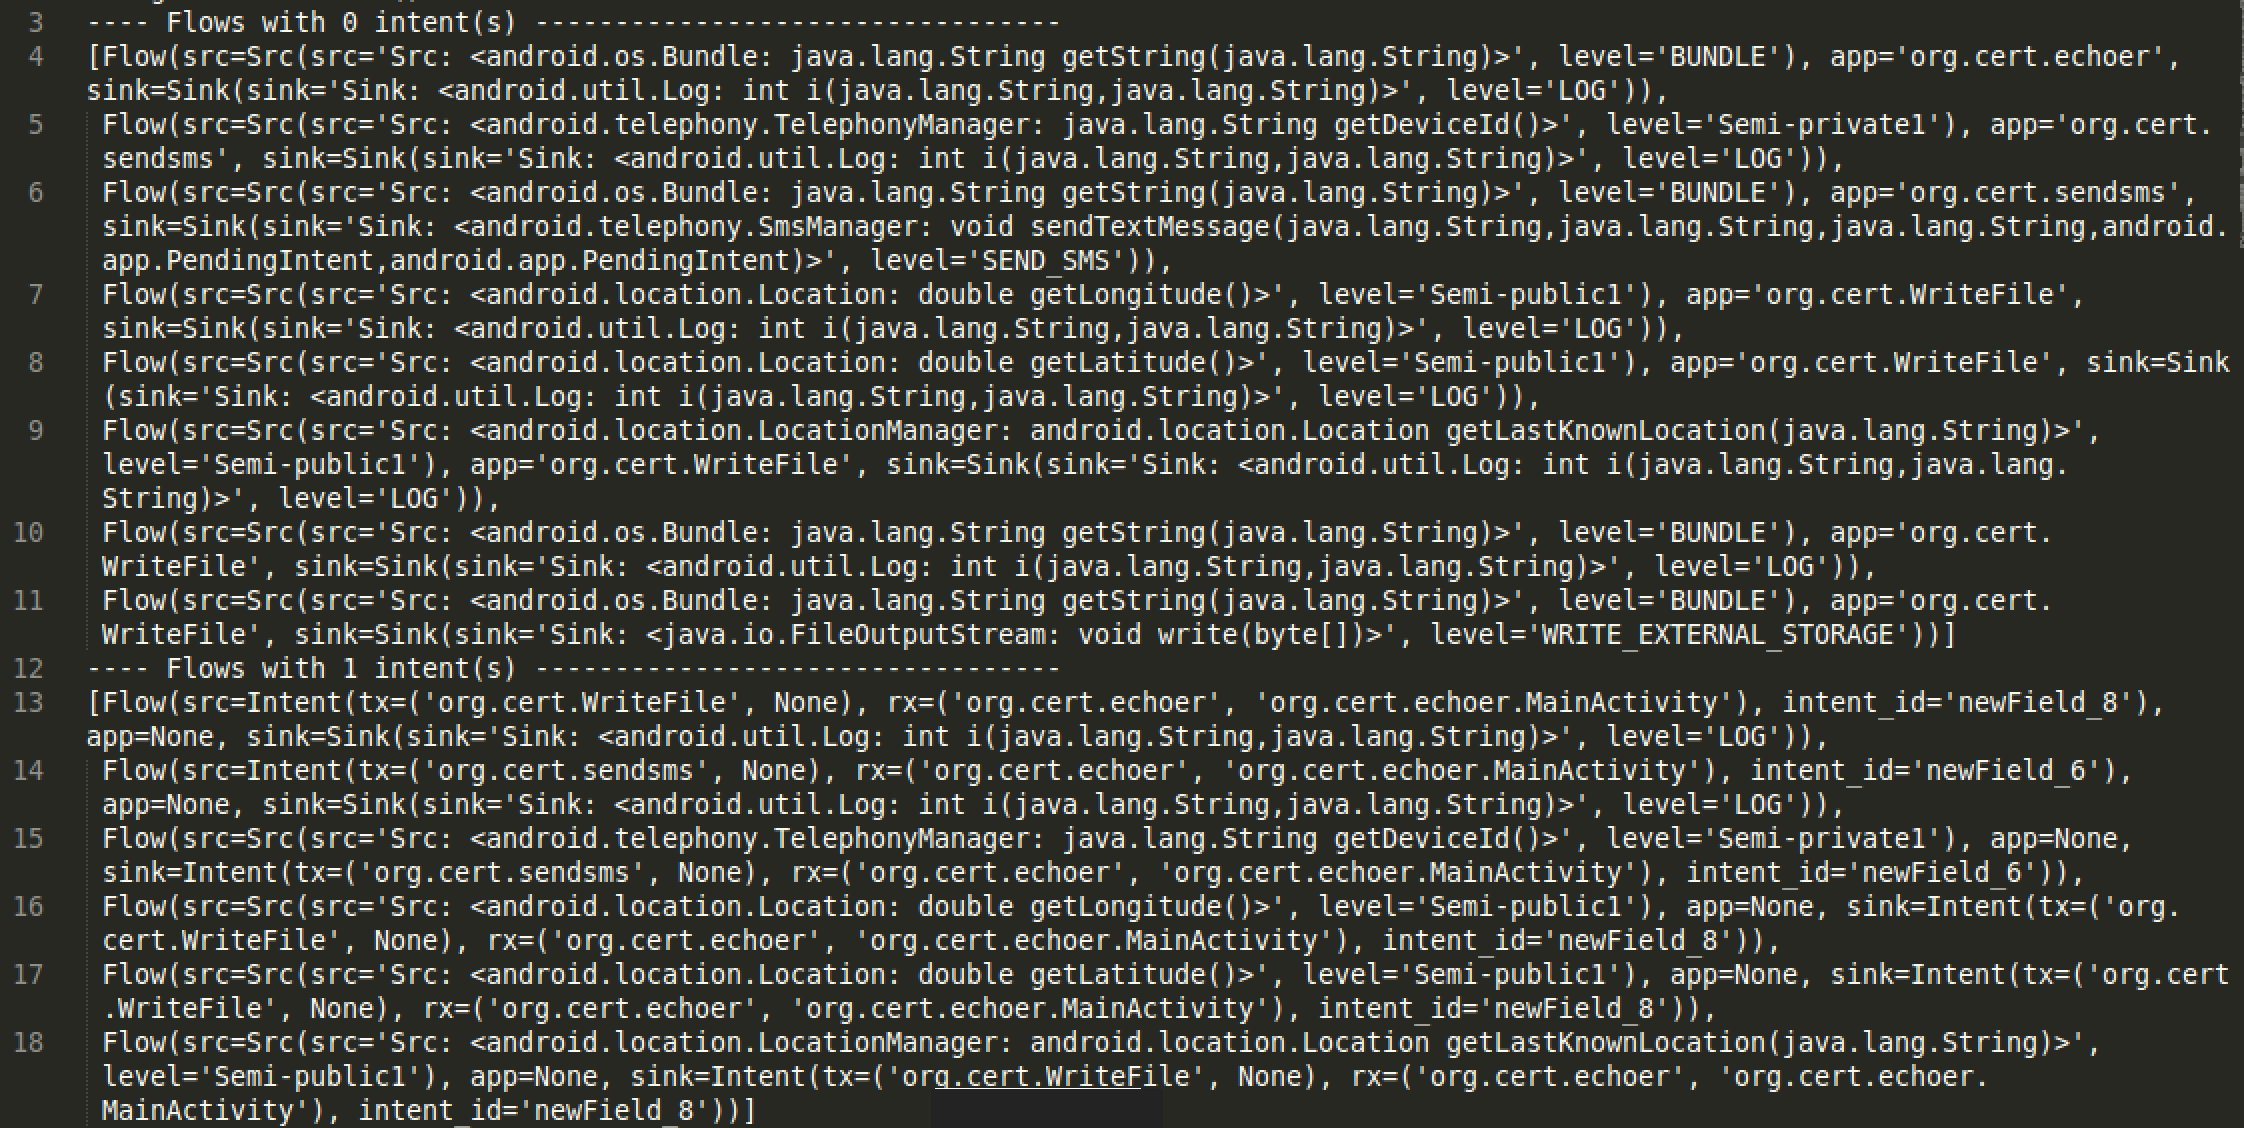
\includegraphics[scale=0.9]{Figura21}
\end{center}

El nivel asignado a la categor�a Log merece una aclaraci�n. Como se mencion� en la descripci�n de las aplicaciones a analizar, al Log le llega informaci�n desde dos lugares, el device Id del usuario con un nivel de seguridad semi-private1 y la ubicaci�n del dispositivo con nivel semi-public1. Para evitar la violaci�n de seguridad, el Log debe tener un nivel igual o mas privado que sus sources, el cual seria semi-private1 o private. Sin embargo, lo obtenido por la herramienta es semi-public1. Esto ocurre por la excepci�n dada (Figura 19), que ignora el flujo del device Id al log.